\documentclass[class=article,border=5pt,tikz]{standalone}
\usepackage{amsmath}% \text{}
\usetikzlibrary{calc,intersections,through,backgrounds}
\usetikzlibrary{angles,quotes,arrows.meta}
\usetikzlibrary{spy}

\tikzset{fig/.pic={code={%

      % coordinates to be reused
      \coordinate (A) at (0,0);
      \coordinate (B) at (1,0);
      \coordinate (C) at (1,1);
      \coordinate (D) at (0,1);
      \coordinate (P) at (0,0.4);
      \coordinate (Q) at (1,0.4);
      \path [name path=DB] (D) -- (B);
      \path [name path=CP] (C) -- (P);
      \path [name path=DQ] (D) -- (Q);
      \path [name path=CA] (C) -- (A);
      \path [name intersections={of=CA and DB, by=S}];
      \path [name intersections={of=DB and CP, by=W}];
      \path [name intersections={of=DQ and CP, by=N}];
      \path [name intersections={of=CA and DQ, by=E}];
      
      % draw figure
      \begin{scope}
      \draw (A) -- (B) -- (C) -- (D) -- cycle;
      \draw (C) -- (P);
      \draw (D) -- (Q);
      \draw (C) -- (A);
      \draw (D) -- (B);
      \end{scope}
                  
      % add labels
      \node [below left] at (A) {A};
      \node [below right] at (B) {B};
      \node [above right] at (C) {C};
      \node [above left] at (D) {D};
      \node [above left] at (P) {P};
      \node [above right] at (Q) {Q};
      
}}}%

\begin{document}
% main figure
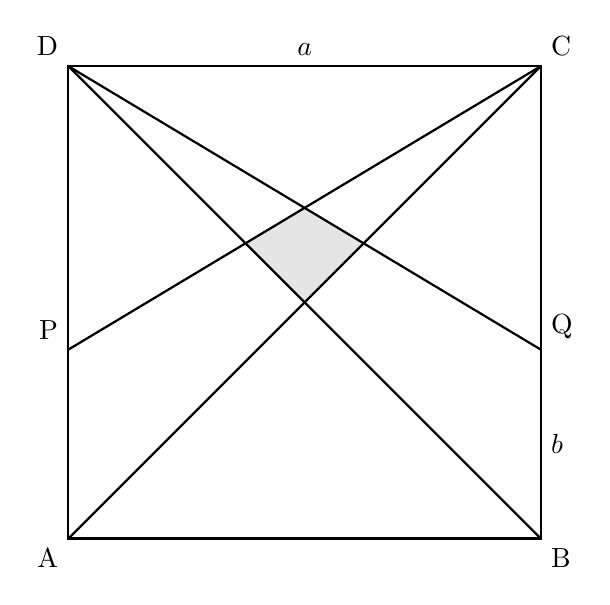
\begin{tikzpicture}[thick, x=6cm, y=6cm]
    \path (0,0) pic {fig};
    \path (C) -- (D) node [midway, above] {$a$};
    \path (B) -- (Q) node [midway, right] {$b$};
    \begin{pgfonlayer}{background}% background otherwise it 'leaks'
      \draw [fill=gray!20] (S) -- (W) -- (N) -- (E);
    \end{pgfonlayer}
\end{tikzpicture}


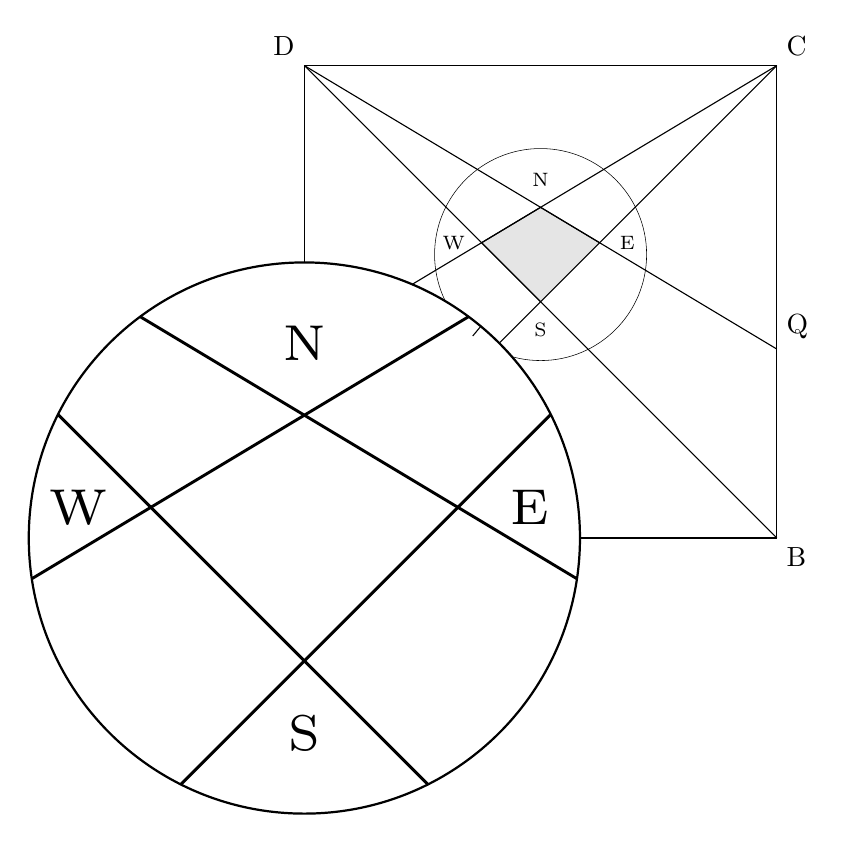
\begin{tikzpicture}[thick, x=6cm, y=6cm, spy using outlines={circle, magnification=2.6, size=7cm, connect spies}]
    \path (0,0) pic {fig};
    \begin{pgfonlayer}{background}% background otherwise it 'leaks'
      \draw [fill=gray!20] (S) -- (W) -- (N) -- (E);
    \end{pgfonlayer}
    % add labels
    \node [shift={(0,-10pt)},font=\scriptsize] at (S) {S};
    \node [shift={(-10pt,0)},font=\scriptsize] at (W) {W};
    \node [shift={(0,10pt)},font=\scriptsize] at (N) {N};
    \node [shift={(10pt,0)},font=\scriptsize] at (E) {E};
    \coordinate (Z) at (0.5,0.6);
    \spy on (Z) in node [fill=white] at (A);
\end{tikzpicture}


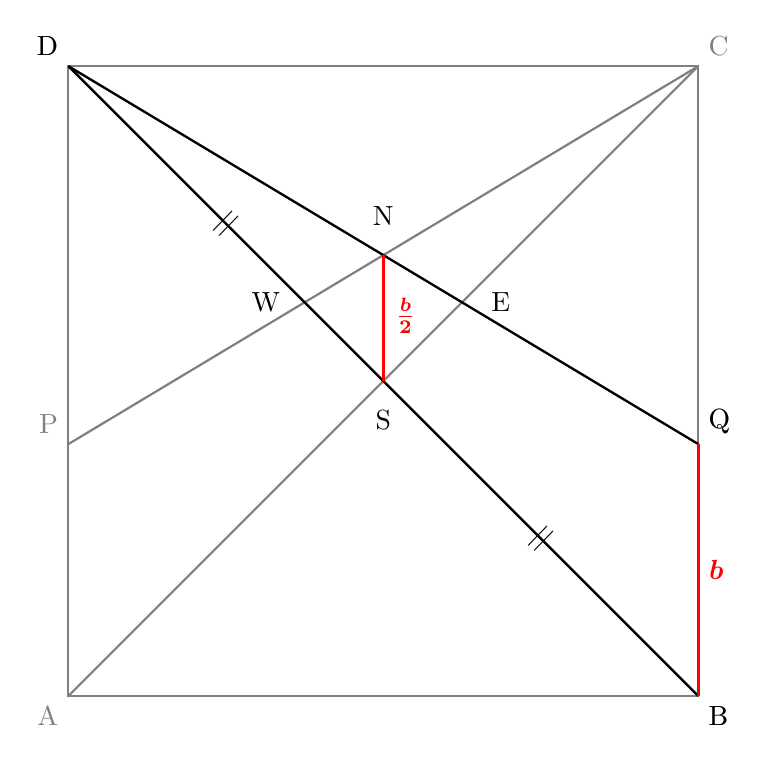
\begin{tikzpicture}[thick, x=8cm, y=8cm]
    \path (0,0) pic[gray] {fig};
    \draw (D) -- (B);
    \draw (D) -- (Q);
    \draw [red,very thick] (B) -- (Q) node [midway, right,font=\boldmath] {$b$};
    \draw [red,very thick] (S) -- (N) node [font=\boldmath,shift={(8pt,-22pt)},fill=white,inner sep=0] {$\frac{b}{2}$};
    \node [above left] at (D) {D};
    \node [below right] at (B) {B};
    \node [above right] at (Q) {Q};
    \node [shift={(0,-14pt)}] at (S) {S};
    \node [shift={(-14pt,0)}] at (W) {W};
    \node [shift={(0,14pt)}] at (N) {N};
    \node [shift={(14pt,0)}] at (E) {E};
    \path (S) -- (B) node [midway,rotate=-44] {$||$};
    \path (D) -- (S) node [midway,rotate=-44] {$||$};
\end{tikzpicture}


\begin{tikzpicture}[thick, x=8cm, y=8cm,double arc/.style={double,double distance=2pt}]
    \draw [gray] (B) -- (D) -- (A) -- (E);
    \draw [gray] (A) -- (B) -- (Q);
    \draw [gray] (C) -- (P);
    % calculate intersection of EW and CQ
    \path [name path=CQ] (C) -- (Q);
    \path [name path=EW] (E) -- (W);
    \path [name intersections={of=EW and CQ, by=E2}];
    \coordinate (E2) at (1,0.625); % above failed, so cheated by guessing E2
    \node [right] at (E2) {E$^{\prime}$};
    \draw [gray,dashed] (E2) -- (W);
    \coordinate (E3) at (0.625,1);
    \node [above] at (E3) {E$^{\prime\prime}$};
    \draw [gray,dashed] (E3) -- (E);     
    \draw pic [draw=red,thick,double arc, angle radius=0.6cm] {angle=E--C--Q};
    \draw pic [draw=red,thick,double arc, angle radius=0.6cm] {angle=D--C--E};
    \draw (D) -- (Q) -- (C) -- (E);
    % add labels
    \node [gray, below left] at (A) {A};
    \node [gray, below right] at (B) {B};
    \node [above right] at (C) {C};
    \node [above left] at (D) {D};
    \node [gray,left] at (P) {P};
    \node [right] at (Q) {Q};
    \node [below] at (S) {S};
    \node [left] at (W) {W\;};
    \node [above] at (N) {N};
    \node [shift={(12pt,0)},fill=white,inner sep=1pt] at (E) {E};
    % tickmarks
    \draw (W|-D) --++(0,3pt);
    \draw (E|-D) --++(0,3pt);
    % (p-|q) = the intersection of a vertical line through p and a horizontal line through q
    \draw (D) -- (W|-D) node [midway,above] {x} -- (E|-D) node [midway,above] {w}-- (Q|-D) node [midway,above] {x}; 
    % add labels for w and w
    \coordinate (W2) at (0.375,1);
    \draw [gray,dashed] (W) -- (W2);
    \coordinate (E4) at (0.625,1);
    \draw [gray,dashed] (E) -- (E4);
    
\end{tikzpicture}


\begin{tikzpicture}[thick, x=8cm, y=8cm]
    % define coordinates (again, for clarity)
    \coordinate (E2) at (1,0.625);
    \coordinate (E3) at (0.625,1);    
    % label points
    \node [above right] at (C) {C};
    \node [above left] at (D) {D};
    \node [below right] at (Q) {Q};
    \node [below] at (E) {E};
    \node [below right] at (E2) {E$^{\prime}$};
    \node [above] at (E3) {E$^{\prime\prime}$}; 
    % draw lines, label distances
    \draw [blue,very thick] (D) -- (E3) node [midway,above,font=\boldmath] {$a-x$};
    \draw [blue,very thick] (E3) -- (C) node [midway,above,font=\boldmath] {$x$};
    \draw (D) -- (Q);
    \draw [red,very thick] (C) -- (Q);    
    \draw [red,very thick] (E) -- (E3);
    \draw [gray,dashed] (E) -- (E2)  node [midway,below] {$x$};
    \path (C) -- (Q) node [midway,shift={(20pt,0pt)},font=\boldmath,red] {$a-b$};
    \path (E) -- (E3) node [midway,right,font=\boldmath,red] {$x$};
\end{tikzpicture}


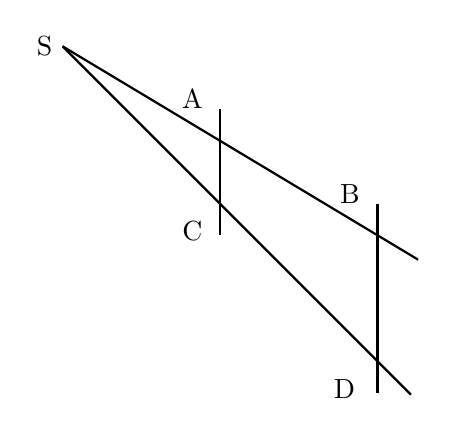
\begin{tikzpicture}[thick,x=4cm, y=4cm]
    % set coordinates
    \coordinate (S) at (0,1);
    \coordinate (A) at (0.5,0.7);
    \coordinate (B) at (1,0.4);
    \coordinate (C) at (0.5,0.5);
    \coordinate (D) at (1,0);
    % draw figure
    \draw [shorten >=-0.6cm] (S) -- (B) node [inner sep=0.6cm] {};% fix to the bounding box that is not extended by shorten >=-0.6cm
    \draw [shorten >=-0.6cm] (S) -- (D);
    \draw [shorten >=-0.4cm,shorten <=-0.4cm] (A) -- (C);
    \draw [shorten >=-0.4cm,shorten <=-0.4cm] (B) -- (D);
    % add labels
    \node [left] at (S) {S};
    \node [shift={(-10pt,+15pt)}] at (A) {A};
    \node [shift={(-10pt,+15pt)}] at (B) {B};
    \node [shift={(-10pt,-10pt)}] at (C) {C};
    \node [shift={(-12pt,-10pt)}] at (D) {D};
\end{tikzpicture}


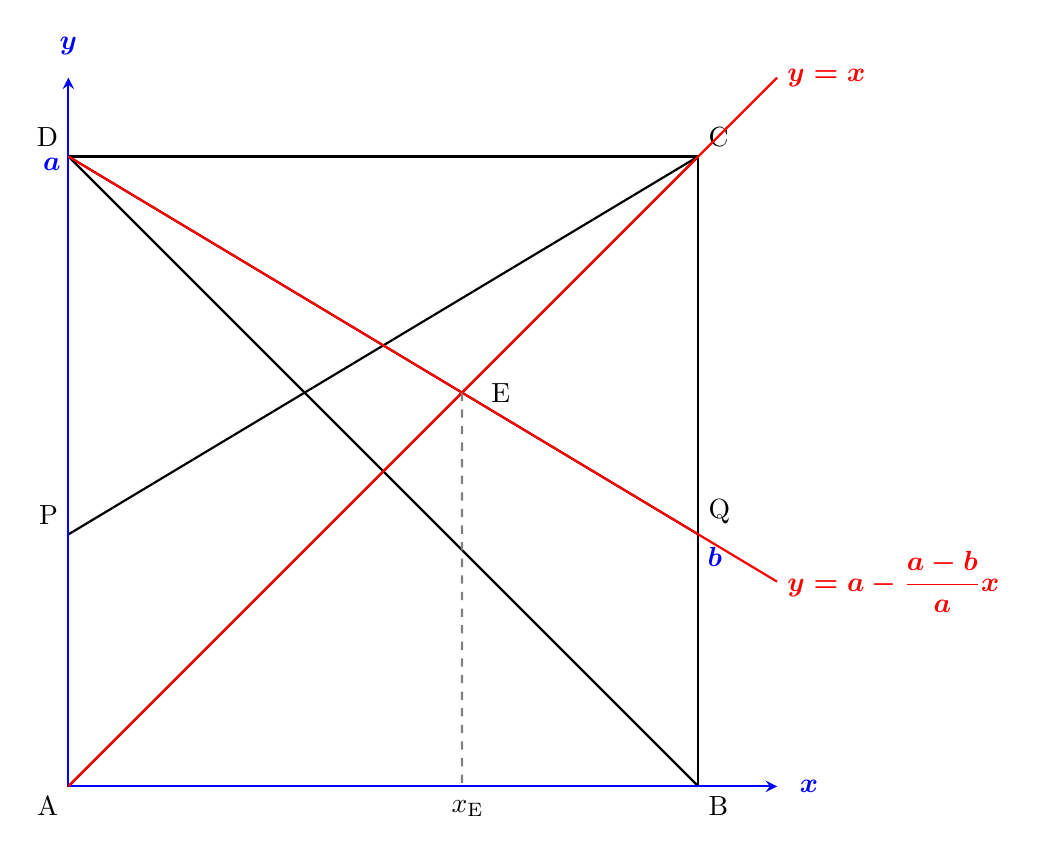
\begin{tikzpicture}[thick, x=8cm, y=8cm]
    \path (0,0) pic {fig};
    \node [shift={(-6pt,-3pt)},blue,font=\boldmath] at (D) {$a$};
    \node [shift={(+6pt,-8pt)},blue,font=\boldmath] at (Q) {$b$};
    \draw [thick,blue,->,>=stealth] (A) -- (B) --++(1cm,0);
    \draw [thick,blue,->,>=stealth] (A) -- (D) --++(0,1cm);
    \node [shift={(40pt,0)},blue,font=\boldmath] at (B) {$x$};
    \node [shift={(0,40pt)},blue,font=\boldmath] at (D) {$y$};
    \node [shift={(14pt,0)}] at (E) {E};
    \draw [thick,red] (A) -- (C) --++(1cm,1cm) node [right,font=\boldmath] {$y=x$};
    \draw [thick,red] (D) -- (Q)--++(1cm,-0.6cm) node [right,font=\boldmath] {$y=a-\dfrac{a-b}{a}x$};
    \coordinate (xE) at (0.625,0);
    \draw [dashed,gray] (E) -- (xE) node [shift={(2pt,-8pt)},black] {$x_{\text{E}}$};
\end{tikzpicture}


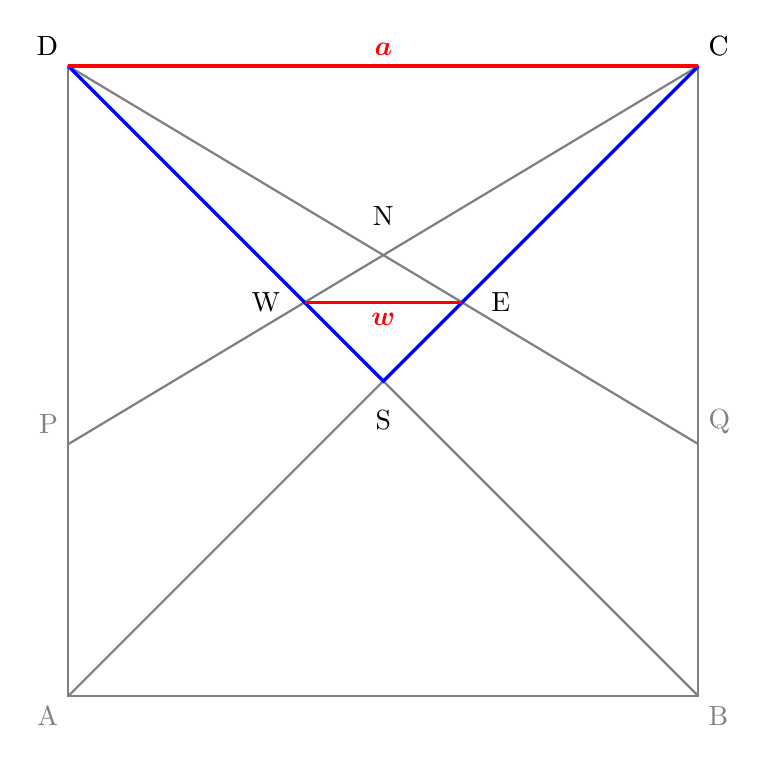
\begin{tikzpicture}[thick, x=8cm, y=8cm]
    \path (0,0) pic[gray] {fig};
%    \coordinate (N2) at (0.5,1);
%    \draw [blue,very thick] (S) -- (N2);
    \draw [blue,very thick] (D) -- (S) -- (C);
    \draw [red,very thick] (W) -- (E) node [midway, below,font=\boldmath,fill=white] {$w$};
    \draw [red,very thick] (D) -- (C) node [midway, above,fill=white,font=\boldmath] {$a$};
%    \node [above] at (N2) {N$^{\prime}$};
    \node [above left] at (D) {D};
    \node [above right] at (C) {C};
    \node [shift={(0,-14pt)}] at (S) {S};
    \node [shift={(-14pt,0)}] at (W) {W};
    \node [shift={(0,14pt)},fill=white] at (N) {N};
    \node [shift={(14pt,0)}] at (E) {E};
\end{tikzpicture}


\end{document}
